\chapter{State of the art}
W celu dokładnego poznania problemu i poprawnego opisania celu pracy zostały o\-mó\-wio\-ne następujące dziedziny badań:
\begin{itemize}
    \item systemy wspomagania decyzji w przedsiębiorstwach produkcyjnych, a zwłaszcza w odlewniach,
    \item algorytmy stosowane w przewidywaniu właściwości materiałów przy użyciu danych,
    \item wykorzystanie algorytmów heurystycznych w celu optymalizacji procesu produkcji.
\end{itemize}

Dodatkowo, w sekcji \ref{sec:ml_algs} zostały opisane algorytmy uczenia maszynowego, które zostały użyte w tej pracy.

\section{Wspomaganie decyzji w przedsiębiorstwach produkcyjnych, od\-lew\-niach}
Pierwsza z omawianych prac \cite{LEGIEN2017897} odnosi się bezpośrednio do problemu wyboru odpowiedniej technologii dla produkcji żeliwa ausferrytycznego sferoidalnego (ADI) w odlewni. Została w niej opracowana architektura wieloagentowa dla systemu wspomagania decyzji, która jest agentową implementacją etykietowanego systemu dedukcyjnego (Labelled Deduction System). Agenci zostali tutaj użyci do dekompozycji systemu do dwóch ortogonalnych wymiarów: dystrybucji wiedzy oraz jej przetwarzania.

Następna z prac \cite{kozlak_2019_agenty}, także nawiązująca do produkcji żeliwa ausferrytycznego sfe\-ro\-idal\-nego, przedstawia wieloagentowy system wspomagający decyzje oraz optymalizujący koszt produkcji wykorzystując różne techniki uczenia maszynowego (Multilayer Perceptron, Random Forest i inne). Do podejmowania kluczowych decyzji zostały wykorzystane dane o udarności próbek żeliwa ADI \cite{Wilk-Kolodziejczyk2018}, która jest bezpośrednio skorelowana z jakością stopu. 

\section{Algorytmy uczenia maszynowego}\label{sec:ml_algs}
W sekcji \ref{sec:model} zostały zaproponowane 4 algorytmy uczenia maszynowego, które chciałbym tutaj dokładnie opisać. Trzy z nich, czyli Random Forest, Gradient Boosting i Ensemble Averaging, należą do algorytmów z rodziny 'ensemble learning'. 

\subsection{Random Forest}
Algorytm Random Forest należy do metod typu 'ensemble learning' czyli takich, które generują wiele prostych modeli i agregują ich wyniki. W przypadku tego algorytmu, tymi prostymi modelami są drzewa decyzyjne. Algorytm ten został zaproponowany przez Breimana \cite{random_forest}. Polega on na dodatniu dodatkowej warstwy losowości do algorytmu Bagging \cite{bagging}. Oprócz konstruowania każdego drzewa przy użyciu innej próbki danych typu bootstrap, lasy losowe zmieniają sposób konstruowania drzew klasyfikacyjnych lub regresyjnych. W drzewach decyzyjnych każdy węzeł jest dzielony przy użyciu najlepszego podziału spośród wszystkich zmiennych. W losowym lesie każdy węzeł jest dzielony przy użyciu najlepszego z podzbioru predyktorów losowo wybranych w tym węźle. Ta nieco sprzeczna z intuicją strategia okazuje się działać bardzo dobrze w porównaniu z wieloma innymi klasyfikatorami, w tym analizą dyskryminacyjną, maszynami wektorów wsparcia i sieciami neuronowymi, i jest odporna na nadmierne dopasowanie \cite{random_forest}. 

\subsection{Gradient Boosting}
Algorytm Gradient Boosting jest następnym przykładem metody typu 'ensemble learning'. Jest jedną z najlepszych technik budowania modeli predykcyjnych. Gradient Boosting jest generalizacją algorytmu AdaBoost \cite{adaboost}. Został stworzony i opisany przez Friedmana \cite{gradient_boosting} w 1999. Aktualnie najnowszą wersją Gradient Boostingu jest XGBoost (Extreme Gradient Boosting), który został zaproponowany w 2016 roku przez Tiangi Chen \cite{xgboost}. Jest to ponownie metoda wykorzystująca wiele prostych modeli, którymi są drzewa decyzyjne i ostateczny wynik zależy od nich wszystkich. XGBoost korzysta ze strategii przyrostowej, gdyż jest to zadanie prostsze i mniej czasochłonne niż wytrenowanie na raz wszystkich drzew. Innowacją w stosunku do algorytmu Friedmana jest wprowadzenie regularyzacji. Została ona zastosowana jako kara za zbyt dużą liczbę liści w drzewie decyzyjnym. W taki właśnie sposób zapewniona jest kontrola złożoności modelu. 

\subsection{Ensemble Averaging}
Algorytm Ensemble Averaging \cite{ensemble_averaging} jest ponownie przykładem metody typu 'ensemble learning' lecz w tym wypadku jest on sposobem na łączenie wielu modeli w jeden. Często takie modele nazywa się modelami komitetu. W skład takich modeli mogą wchodzić modele wytrenowane przy pomocy różnych algorytmów albo modele wytrenowane za pomocą tego samego algorytmu lecz różniące się od siebie np.  poprzez wytrenowanie ich za pomocą różnych wartości parametrów wejściowych.

Najprostszym sposobem na łączenie modeli jest przedstawianie wyjścia takiego modelu jako średnią wartość z wyjść modeli wchodzących w skład komitetu. Drugą możliwością jest nadawanie wag wartościom wyjściowym z modeli, które to wagi mogą być związane np. z jakością modelu.

\subsection{Multilayer Perceptron}
Multilayer Perceptron \cite{negnevitsky2005artificial} czyli perceptron wielowarstwowy to sieć neuronowa w pełni połączona typu feed-forward, która jest tak naprawdę piętrową wersją perceptronu jedno-warstwowego. W przeciwieństwie do perceptronów jedno-warstwowych, jest używana do rozwiązywania problemów nieliniowych. Funkcje aktywacji zdefiniowane w warstwach umożliwiają sieciom opartym na wielowarstwowych perceptronach uzyskanie modelu nieliniowego. Każdy perceptron wielowarstwowy składa się z przynajmniej 3 warstw. Pierwszą z nich jest warstwa nazywana wejściową, która przyjmuje wektor wartości wejściowych. Następną warstwą jest warstwa ukryta przez którą przechodzą informacje z warstwy wejściowej do następnej warstwy ukrytej bądź do warstwy wyjściowej. Ostatnia warstwa, nazywana warstwą wyjściową, zwraca nam wartości przewidywane przez sieć.

Uczenie takiej sieci odbywa się przy użyciu algorytmu wstecznej propagacji błędu i stochastycznego spadku wzdłuż gradientu.

\section{Podejścia do przewidywania właściwości wyrobów produkcyjnych}
Przewidywanie właściwości wyrobów produkcyjnych (np. produkcja żeliw) polega na zbudowaniu modelu, który dla ustalonych parametrów produkcji (np. skład produkowanego żeliwa czy parametry jego obróbki) zwróci jego właściwości (np. mechaniczne), które są istotne z punktu widzenia odbiorcy wyrobu. Poniższy przegląd skupia się głównie na przewidywaniu właściwości mechanicznych żeliwa ADI. Modele przewidujące te właściwości budowane są najczęściej na podstawie danych zbieranych z literatury oraz publikowanych artykułów. Naistotniejszymi właściwościami żeliwa ADI są: wytrzymałość na rozciąganie, elastyczność oraz twardość, które są najczęściej występujacymi w literaturze. Ze względu na to, że badanie twardości jest procesem dość prostym oraz tanim, część artykułów zawiera informację tylko o twardości. Kolejnymi ważnymi parametrami, ale występujacymi rzadziej, są: granica plastyczności oraz udarność. 

Jak już zostało wspomniane powyżej, badanie twardości jest procesem najprostszym i~z~tego względu wyniki twardości są przedstawiane dla największej liczby próbek. Ze względu na ten fakt, większość badań związanych z przewidywaniem właściwości fizycznych żeliwa ADI skupia się tylko na przewidywaniu twardości.

\subsection{Przewidywanie właściwości mechanicznych żeliwa ADI}\label{sec:sota-prediction}
Wszystkie omówione w tym rozdziale prace będą związane z budowaniem modeli do przewidywania jednego bądź wielu właściwości żeliwa ADI. W przypadku tych modeli, w których przewidywana jest więcej niż jedna właściwość, dochodzi do problemów związanych z brakującymi danymi dla jednej z nich. Problem ten został przedstawiony w pracy A. Kochańskiego i innych \cite{Kochanski12} gdzie zostało zaprezentowane przykładowe rozwiązanie. Mianowicie, w celu uzupełnienia brakujących wartości należy znaleźć podzbiór próbek, w~których dla wymiaru, w którym brakuje danych, istnieje wysoce skorelowany inny wymiar, na podstawie którego możliwe jest wyznaczenie brakujacej wartości np. za pomocą regresji liniowej. W pracy stwierdzono, że zaletą takiego podejścia jest możliwość uzyskania nowych wartości granicznych zbioru danych. W przypadku, gdy korelacja między atrybutami nie występuje, brakująca wartość może zostać obliczona poprzez porównanie z wybranymi rekordami ze zbioru zawierającego pełne dane.

Jedną z pierwszych prac, która poruszała problem przewidywania właściwości mechanicznych żeliwa ADI, była praca autorów S.K Putatunda i innych \cite{777072}. Zostały w niej opisane różne modele bazujące na logice rozmytej (fuzzy-based model), które zostały zaimplementowane w celu przewidywania udarności żeliwa ADI na podstawie temperatury i czasu trwania procesu ausferryzacji przy założeniu, że pozostałe parametry były stałe. Zbiór danych, na których uczony był model, zawierał tylko 28 próbek, z których 21 zostało wybranych jako zbiór treningowy, a reszta, czyli 7 próbek, jako zbiór testowy. Najlepszy wynik uzyskało podejście oparte na klasteryzacji, w którym współczynnik korelacji wartości przewidzianych do rzeczywistych wyniósł 0,9. 

Następna z prac, autorstwa Miguela Yescasa \cite{doi:10.1080/13640461.2003.11819537}, przedstawia przewidywanie twardości żeliwa ADI przy użyciu sieci neuronowych. Jest to pierwsza z prac znalezionych w literaturze, która podejmuje ten problem. Stosując takie podejście, został opracowany model komitetu bayesowskich sieci neuronowych. Sieci te budowane były przy użyciu jednej warstwy ukrytej, dla której testowane były różne liczby neuronów - od 2 do 20, oraz różne stałe regularyzacji (jedna powiązana z każdym wejściem, jedna z biasami i jedna dla wag połączonych z wyjściem). Zostały także przetestowane różne liczby najlepszych konfiguracji sieci wchodzących w skład komitetów. 

Proces uczenia sieci został przeprowadzony przy użyciu zbioru zawierającego 1822 próbki zebrane z literatury. Zbiór został podzielony losowo na treningowy i testowy w~proporcji 50/50. Wejściem wszystkich sieci był zestaw składu chemicznego wytopów, parametry ich obróbki cieplnej oraz przedstawienie czasu ausferrytyzacji za pomocą logarytmu wartości czasu w sekundach. Takie podejście zostało opracowane w pracy tego samego autora, która dotyczyła wyznaczania zawartości zachowanego austenitu w żeliwie ADI \cite{YESCAS2001162}. Wymiary wejściowe sieci zostały poddane normalizacji do zakresu [-0,5;0,5].

Badania wykazały, że im więcej neuronów w warstwie ukrytej, tym poziom zaszumienia jest mniejszy (rys. \ref{fig:vhn-pred-mae-plot}). Niewielki wpływ miały także różne stałe regularyzacji (wyniki różnych konfiguracji przedstawione za pomocą plusów). Na podstawie prawej części wyżej wspomnianego wykresu można określić, że wartość błędu najlepszych modeli oscyluje między 1,5 a 2.

\begin{figure}[ht]{}
	\centering
	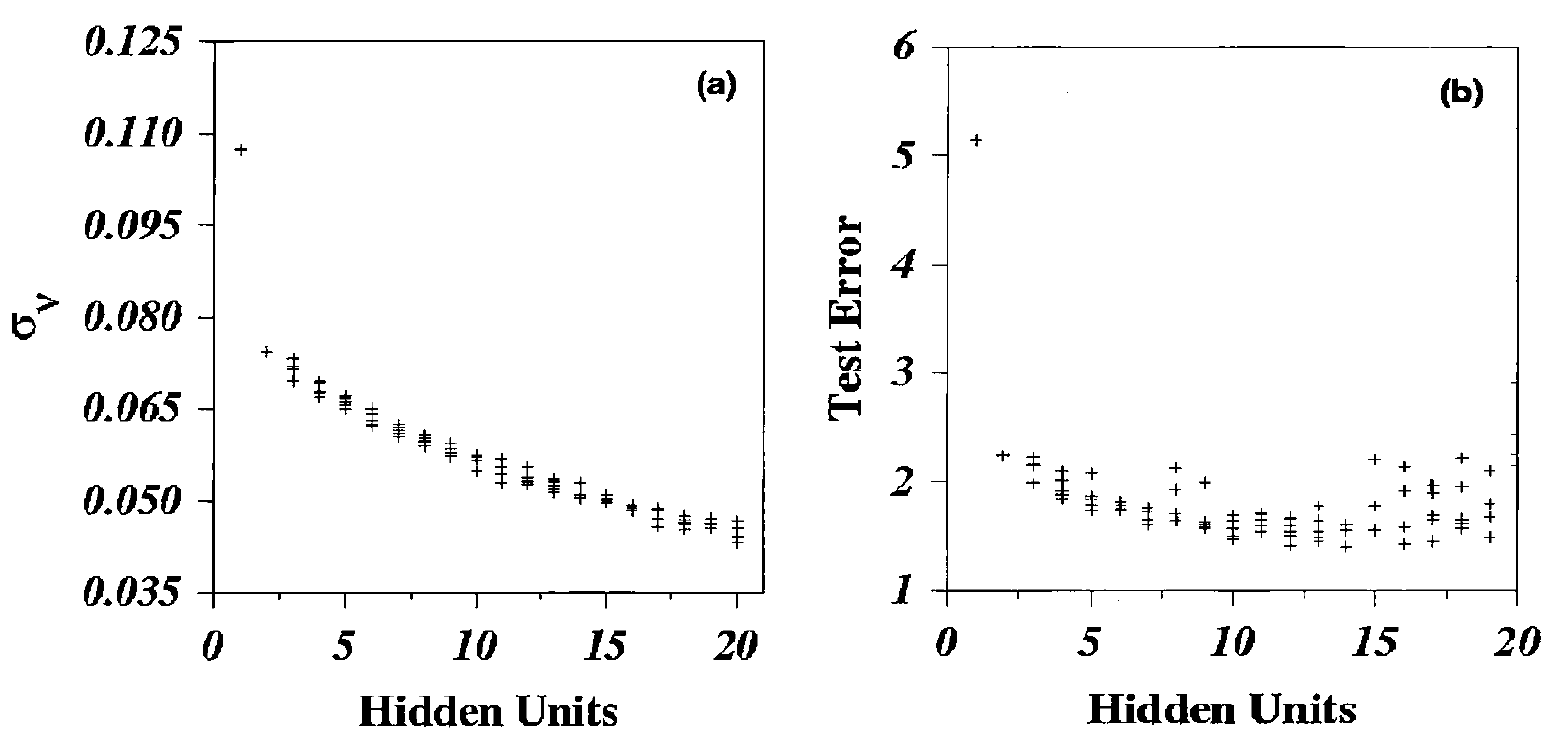
\includegraphics[scale=0.35]{images/vhn-test-error-plot.png}
	\caption {
		 Po lewej wykres zależności poziomu szumu od liczby neuronów w warstwie ukrytej, po prawej wykres zależności błedu predykcji od liczby neuronów w warstwie ukrytej, wykresy pochodzą z pracy \cite{doi:10.1080/13640461.2003.11819537}
	}
	\label{fig:vhn-pred-mae-plot}
\end{figure}

Dalsze badania były oparte na budowie komitetu modeli, w którym wynik przedstawiony był jako średnia wartość predykcji modeli wchodzących w jego skład. Badane komitety były budowane z modeli, które osiągały najlepsze wyniki w badaniach liczby neuronów oraz stałych regularyzacji. Wyniki badania zostały przedstawione na rys. \ref{fig:committee-plot}. Badacze stwierdzili, że najlepszym komitetem okazał się ten składający się z 10 najlepszych modeli, co widać na wyżej wspomnianym rysunku.

\begin{figure}[ht]{}
	\centering
	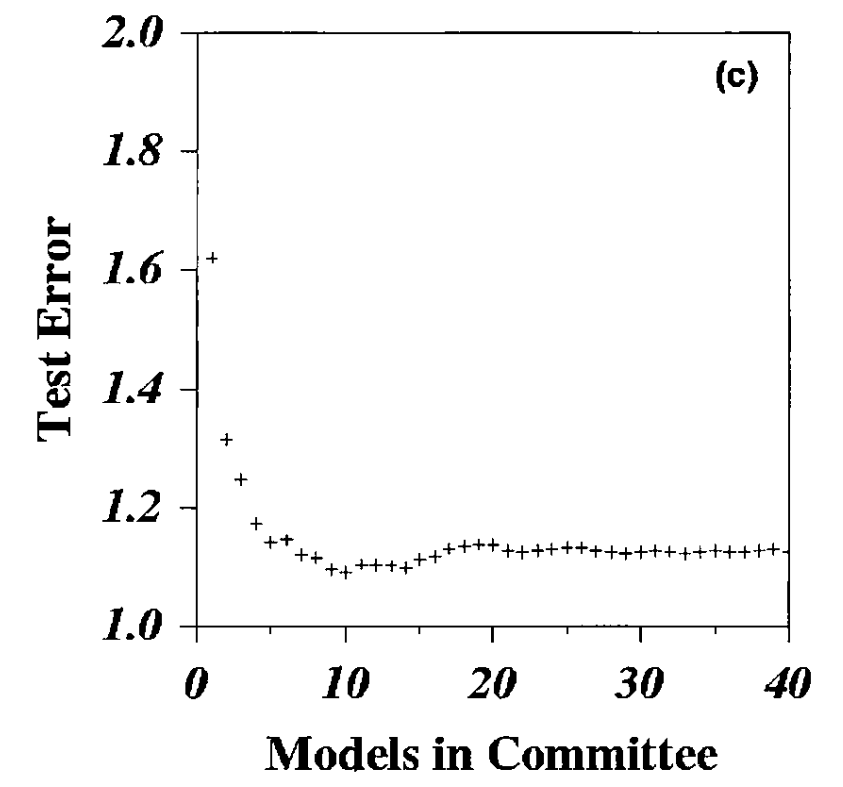
\includegraphics[scale=0.35]{images/committee-plot.png}
	\caption {
		 Wykres zależności błędu predykcji od liczby modeli wchodzących w skład komitetów \cite{doi:10.1080/13640461.2003.11819537}
	}
	\label{fig:committee-plot}
\end{figure}

Budowa modeli predykcyjnych twardości została także przedstawiona w pracach \cite{POURASIABI2012782}, \cite{10.1007/978-3-030-36802-9_43}, \cite{10.1007/978-3-030-36802-9_44}, gdzie prace \cite{10.1007/978-3-030-36802-9_43} i \cite{10.1007/978-3-030-36802-9_44}, autorów Savagounder'a, Patra i Bornanda, zostały opublikowane równolegle, bazując na danych, które zostały przedstawione w \cite{POURASIABI2012782}. Wspomniany zbiór danych zawiera 96 próbek zróżnicowanych pod względem składu chemicznego oraz parametrów obróbki cieplnej. Został on sporządzony na podstawie badań twardości żeliwa ADI, których procedura została ściśle opisana w artykule.

W pracy Hamida oraz Hameda PourAsiabi i innych \cite{POURASIABI2012782}, model predykcyjny został opracowany w sposób przedstawiony na rys. \ref{fig:sch-vhn-pourasiabi}. Jest to model sieci neuronowej, w~której warstwa wejściowa składa się z: wartości proc. miedzi i molibdenu oraz temperatury i czasu ausferrytyzacji. Warstwa ukryta składa się z 5 neuronów, w której funkcją aktywacji jest funkcja tangensoidalna. Zbiór danych został podzielony na zbiór treningowy oraz testowy w proporcji 70/26. Do minimalizacji błędu sieci została użyta metoda błędu średniokwadratowego, a dla uzyskania optymalnych wag został użyty algorytm Levenberga-Marquardta, bazujący na pochodnej drugiego rzędu funkcji błędu. Została także zastosowana normalizacja wymiarów wejściowych do wartości z zakresu [-1,1].


\begin{figure}[ht]{}
	\centering
	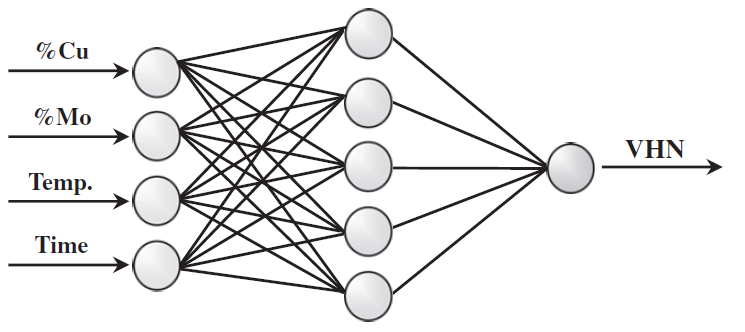
\includegraphics[scale=0.5]{images/model_vhn_pourasiabi.png}
	\caption {
		 Schemat modelu sieci neuronowej przedstawionego w pracy \cite{POURASIABI2012782}.
	}
	\label{fig:sch-vhn-pourasiabi}
\end{figure}

Wyniki testów wytrenowanej sieci neuronowej zostały przedstawione za pomocą współczynnika korelacji, którego wartość wyniosła 0.9912. Tak wysoki wynik świadczy o~dobrze wytrenowanej sieci oraz zdolności do poprawnego przewidywania twardości.

% \cite{adi-pred-2006}
% \cite{adi-pred-2014}

% \subsection{Inne wybrane modele predykcyjne}
% \label{sec:other-pred}
% \cite{ai_heat_treatment}
% \cite{GUO201995}
% \cite{4344283}

\section{Opis wybranych algorytmów heurystycznych}
W tej sekcji zostały przedstawione algorytmy heurystyczne, ktore zostały użyte na potrzeby optymalizacji parametrów produkcji żeliwa ADI (sekcja \ref{sec:algos}). Należą one do rodziny algorytmów przeszukiwania lokalnego ze względu na wykorzystanie sąsiedztwa wartości parametrów.

\subsection{Hill Climbing i Stochastic Hill Climbing}
Algorytm Hill Climbing \cite{hillclimbing} jest algorytmem przeszukiwania lokalnego zachłannego (nazywany też wspinaniem wzdłuż gradientu). Dla aktualnego rozwiązania wybierany jest zawsze sąsiad z największą bądź najmniejszą wartością funkcji celu w zależności od czego czy rozpatrywany jest problem minimalizacji bądź maksymalizacji. Wadą tego algorytmu jest zatrzymywanie się w w minimach/maksimach lokalnych. Algorytm Stochastic Hill Climbing jest modyfikacją poprzedniego algorytmu, która dokłada losowość. W tym algorytmie następne rozpatrywane rozwiązanie jest losowane z dostępnych sąsiadów do póki któryś z nich nie okaże się lepszy od aktualnego. Algorytm nie posiada określonego kryterium stopu więc należy zastosować np. maksymalny czas przeszukiwania bądź maksymalną liczbę kroków.

\subsection{Tabu Search}
Algorytm Tabu Search \cite{tabusearch} realizuje mechanizm, który nie pozwala zatrzymywać się przeszukiwaniu w ekstremach lokalnych. Oparty jest na redukcji przestrzeni przeszukiwań o znalezione rozwiązania. Podczas działania algorytmu używana jest tablica tabu, która na początku jest pusta. Do tablicy dodajemy rozwiązanie, które okazuje się gorsze od wybranego sąsiada. Zbiór wygenerowanych sąsiadów jest w każdym kroku algorytmu uszczuplany o rozwiązania znajdujące się w tablicy tabu. Rozwiązania są usuwane z tablicy tabu po pewnej określonej liczbie iteracji. Nie posiada on naturalnego warunku zakończenia. Wadą tego algorytmu jest przetrzymywanie w pamięci tablicy tabu.

Algorytm Tabu Search można zaimplementować na dwa sposoby:
\begin{itemize}
    \item uniemożliwienie generowania nowych rozwiązań, które są w tablicy tabu,
    \item nowe rozwiązanie nie może zostać wybrane, jeśli znajduje się w tablicy tabu.
\end{itemize}

Złamanie tablicy tabu dopuszczalne jest w przypadku, gdy wszyscy sąsiedzi danego rozwiązania znajdują się w tablicy tabu.

\subsection{Metropolis Search}
Algorytm Metropolisa \cite{metropolis} jest algorytmem statystycznego symulowania zmian ciała stałego w gorącej kąpieli aż do stanu termicznej równowagi. Przeszukiwanie odbywa się w następujący sposób:
\begin{itemize}
    \item dla danego rozwiązania \textit{i} wykonujemy statystyczny 'ruch' cząstki, otrzymując rozwiązanie \textit{j},
    \item jeżeli $E_{j}-E_{i} < 0$ (E - energia rozwiązania) to wybieramy rozwiązanie \textit{j},
    \item w przeciwnym wypadku wybieramy rozwiązanie \textit{j} z prawdopodobieństwiem \\* $exp\Big(-\frac{E_{j}-E_{i}}{k_{b}T}\Big)$
    \item wykonujemy kolejny statystyczny 'ruch'.
\end{itemize}

Algorytm nie posiada kryterium stopu, należy zastosować maksymalny czas bądź maksymalną liczbę kroków.

\section{Algorytmy heurystyczne w optymalizacji pro\-ce\-su pro\-du\-kcji}

Pierwszą z omówionych prac jest praca autorstwa A. Kumara i innych \cite{doi:10.1002/srin.201100189}, w której została zastosowana optymalizacja Pareto przy użyciu algorytmów genetycznych w oparciu o zbiór danych. Przedmiotem optymalizacji były właściwości mechaniczne stali mikrostopowej, a dokładniej: wytrzymałość na rozciąganie, wydłużenie oraz granica plastyczności. Na potrzeby optymalizacji zostały stworzone modele właściwości mechanicznych oparte na ewolucyjnych sieciach neuronowych (EvoNN). W pracy została przeprowadzona optymalizacja wielokryterialna oparta na optymalizacji następujących zestawów kryteriów:
\begin{itemize}
    \item maksymalizacji wytrzymałości na rozciąganie oraz granicy plastyczności,
    \item maksymalizacji granicy plastyczności oraz wydłużenia,
    \item maksymalizacji granicy plastyczności oraz minimalizacji stosunku granicy plastyczności do wytrzymałości na rozciąganie.
\end{itemize}
Trzy powyższe zadania optymalizacji zostały przeprowadzone z użyciem wielo-kryterialnego algorytmu genetycznego o nazwie 'predator-prey'. Rozwiązania Pareto dla każdego z zadań optymalizacyjnych odbiegały znacząco od rozwiązań opartych na danych użytych do budowy modeli. Aby sprawdzić tę bardzo istotną obserwację, przygotowano stop w bliskim sąsiedztwie kompozycji uzyskanej z frontu Pareto, która zgodnie z wiedzą badaczy nie była do tej pory przez nikogo badana. Próbki pochodzące z przygotowanego stopu zostały zbadane i ich właściwości (w granicy błędów eksperymentalnych) były całkiem zgodne z frontem Pareto. Badacze ocenili, że stworzenie stali o lepszych kombinacjach właściwości niż którykolwiek z elementów ze zbioru danych byłoby niemożliwe do uzyskania poprzez wykonanie samych eksperymentów, a udało się uzyskać taką kombinację za pomocą optymalizacji wielokryterialnej.

Następną z prac omawiających optymalizację procesu produkcji jest praca autora R. Radisa i innych \cite{radivsa2017casting}, w której badacze podjeli się problemu optymalizacji geometrii podajnika służącego do odlewania łyżki turbiny Peltona. Utworzona funkcja celu została opracowana na podstawie wymogów transferu ciepła. Zostały także opracowane 4 różne wymagania dla rozwiązań zwracanych przez algorytmy optymalizacji. Optymalizacji zostały poddane 4 różne wartości (H, R, r, l) przy użyciu 4 różnych algorytmów metaheurystycznych: algorytmu genetycznego, kolonii mrówek, symulowanego wyżarzania i optymalizacji roju cząstek. Wyniki otrzymane dla każdego z algorytmów okazały się bardzo zbliżone do siebie. Na ich podstawie został zamodelowany podajnik dla którego zostały przeprowadzone symulacje numeryczne potwierdzające poprawność rozwiązania.
